\Chapter{Validáció}

\section{Adathalmaz}

A kézzel írott kínai karakterek sok adatbázisban megjelent, de csak az újabbak célja a nem kényszerített kézírás.

Az új CASIA-OLHWDB és CASIA-HWDB több előnnyel is rendelkeznek: nem kényszerített írás, egyidejű online és offline adatok, elkülönített minták, több kategóriák, nagyszámú írók és minták.

Az online adatkészletek biztosítják a stroke koordinátáinak sorrendjét. Az offline adatkészletek gray-scaled képek, 255 pixel értékű háttérképen.

\subsection{Tanítás és tesztelés}

A tanító mintáknak különböznie kell a tesztelési mintáktól. A tanítási mintahalmazra a hálózat pontossága magasabb, hiszen a tesztelési pontokat nem ismeri.

Az arányok megválasztásába gyakori a 80/20 (tanító/tesztelő) arány. Az én esetemben 4GB tanító 1GB tesztelő adathalmazt használok.

Az offline adatokkal végzem el a tanítást.\Aref{fig:offline_dataset} ábrán láthatunk példát a kínai karakterekre.

\begin{figure}[h]
	\centering
	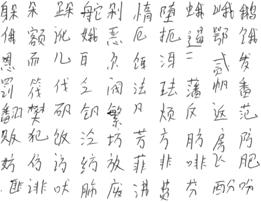
\includegraphics[scale=1.0]{images/offline_dataset}
	\caption{Offline adatbázis példa}
	\label{fig:offline_dataset}
\end{figure} 

Az adathalmaz végig iterálása előtt azokat érdemes össze keverni véletlenszerűen. Ennek eredménye hogy a hálózat minden egyes futtatás során egy picivel máshogy fog tanulni. A különbözöségek elkerülésére lehet használni egy úgynevezett \textit{seed}-et, aminek fixálásakor megegyező módon keveri össze az adatokat.

\begin{python}
random.shuffle(self.image_names)
\end{python}

A keverés mellet véletlenszerű zajokat is hozzáadhatunk a képekhez (vágás, forgatás, elmosás). A zaj hozzáadáshoz a \textit{imgaug} csomag rendkivül hasznos.

\begin{python}
from imgaug import augmenters as iaa

seq = iaa.Sequential([
    iaa.Crop(px=(0, 16)), # vágás 
    iaa.Fliplr(0.5), # horizontális forgatás (50%-ba) 
    iaa.GaussianBlur(sigma=(0, 3.0)) # elmosás 0-3.0 szigma-val
])
\end{python}

A imgaug dokumentációba részletezve vannak az argumentumok (Flipud, Affine, SimplexNoiseAlpha, Dropout, Grayscale, Scale).

\section{Tanítás}

\subsection{Beolvasás}
A tanítás elött be kell olvasni a kínai karaktereinket. Mind a tanító mind a tesztelő adathalmaznak ki kell nyerni a címkéjét, ami meghatároza, hogy a kép milyen karakter.

A különböző zajokkal ellátott képeket külön-külön be lehet tanítani a hálózattal. Ebben az esetben szét kell választani az képeket zajok szerint, majd azokat betölteni. \Aref{fig:noisy_picture} ábrán láthatóak a zajosított képek egy adott karakterre.

\begin{figure}[h]
	\centering
	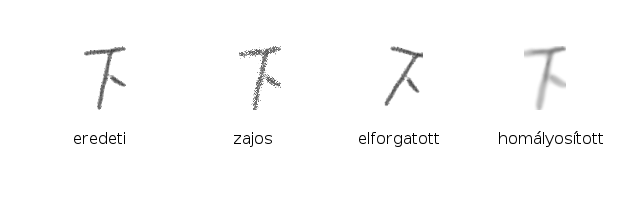
\includegraphics[scale=0.45]{images/pictures_with_noise}
	\caption{Zajosított képek}
	\label{fig:noisy_picture}
\end{figure}

\subsection{Tanítás}

A kép jellemzők kiválasztásához a 4. fejezetben említett konvolúciós hálózatot használom. A CNN a jelenlegi legjobb modellek az objektumok felismerésére, a pontossága 94+\%.

\Aref{fig:arch} a hálózat architektúrát szemlélteti:

\begin{figure}[h]
	\centering
	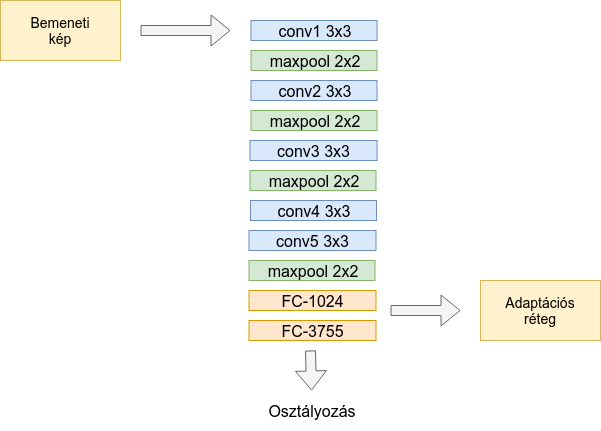
\includegraphics[scale=0.45]{images/architecture}
	\caption{Architektúra}
	\label{fig:arch}
\end{figure}

\begin{itemize}
\item Öt konvolúciós (convolution) réteg. Az első réteg megkapja a képet. A kép 64x64 pixel méretű és 1 szín csatorna (gray-scaled) van. A rétegeken 3x3 szűröt (kernel) használok 1-es lépéssel (stride).
\begin{python}
model.add(Convolution2D(1,	# filter rétegek száma    
                        3, 3,	# 3x3 kernel méret 
                        strides=(1,1) # lépés
                        input_shape=image))
\end{python}
\item Négy összevonó (pooling) réteg. Bemenetei a konvolúciós rétegek kimenetei. A rétegen maximális összevonás (max-pooling) van.
\begin{python}
model.add(MaxPooling2D(pool_size=(2,2)))
\end{python}
\item Két teljesen összekötött (fully-connected) réteg. Az aktivációs függvény: RELU, a dropout: 0.2, neuronok száma: 1024, 3755.
\begin{python}
model.add(Flatten()) # Bemenet
model.add(Dense(1024, activation='RELU'))
model.add(Dropout(0.2))
model.add(Dense(3755, activation='None'))
\end{python}
\end{itemize}

A tanítás a 4. fejezetben említett hiba visszaterjesztéssel (backpropagation) történik. A célunk az hogy a hibát megprobáljuk a minimumra csökkenteni, amit a hálózat súlyainak változtatásával érünk el.

\begin{python}
# Negyzetes hiba
model.compile(loss='mean_squared_error',
              optimizer='adam',
              metrics=['accuracy'])

# Halozat tanitas
model.fit_generator(generator=training_data,
                    steps_per_epoch=1000, epochs=10)
\end{python}

Tesztelés

A validáció ideje körülbelül 17 órát vett igénybe. A hardver: CPU - 4 mag 2.8Ghz, RAM - 4Gb.